%!TEX program = lualatex
\documentclass[a4paper,11pt, twocolumn]{ltjsarticle}

\usepackage{amsmath} % 数式を使うためのパッケージ
\usepackage{graphicx} % 画像を挿入するためのパッケージ
\usepackage{url} % URLを表示するためのパッケージ
\usepackage{fix-cm} % Computer Modernフォントの任意サイズ対応
\usepackage[backend=biber,style=numeric-comp,sorting=none]{biblatex} % [1]形式の引用スタイル
\addbibresource{references.bib} % 参考文献ファイルを指定

\usepackage[top=15mm, left=25mm, right=25mm, bottom=25mm]{geometry}

\title{ 自走式ディスプレイのためのFPGAによるLEDマトリクスコントローラーの実装 }
\author{ 
  Arch junpei \thanks{慶應義塾大学 環境情報学部 2年} \\
  \and
  親: macchan \thanks{慶應義塾大学 政策・メディア研究科 特任講師}
}
\date{}

% \begin{abstract}
% あいうえおかきくけこさしすせそたちつてとあいうえおかきくけこさ
% \end{abstract}

\begin{document}

\maketitle

\section{自走式ディスプレイとは}
自走式ディスプレイとは、ディスプレイを台車の上に搭載することで、画面よりも大きな空間をインタラクティブに表示するデバイスである。デバイスの移動量に応じて、表示内容を動的に変化させることで、ディスプレイを仮想空間への「のぞき窓」\cite{fitzmaurice1993}として機能させる。

筆者は、2023年度から図\ref{fig:display}のような自走式ディスプレイの開発を行ってきた。本稿では、自走式ディスプレイのための、LEDマトリクスコントローラーの実装について述べる。

\begin{figure}
\centering
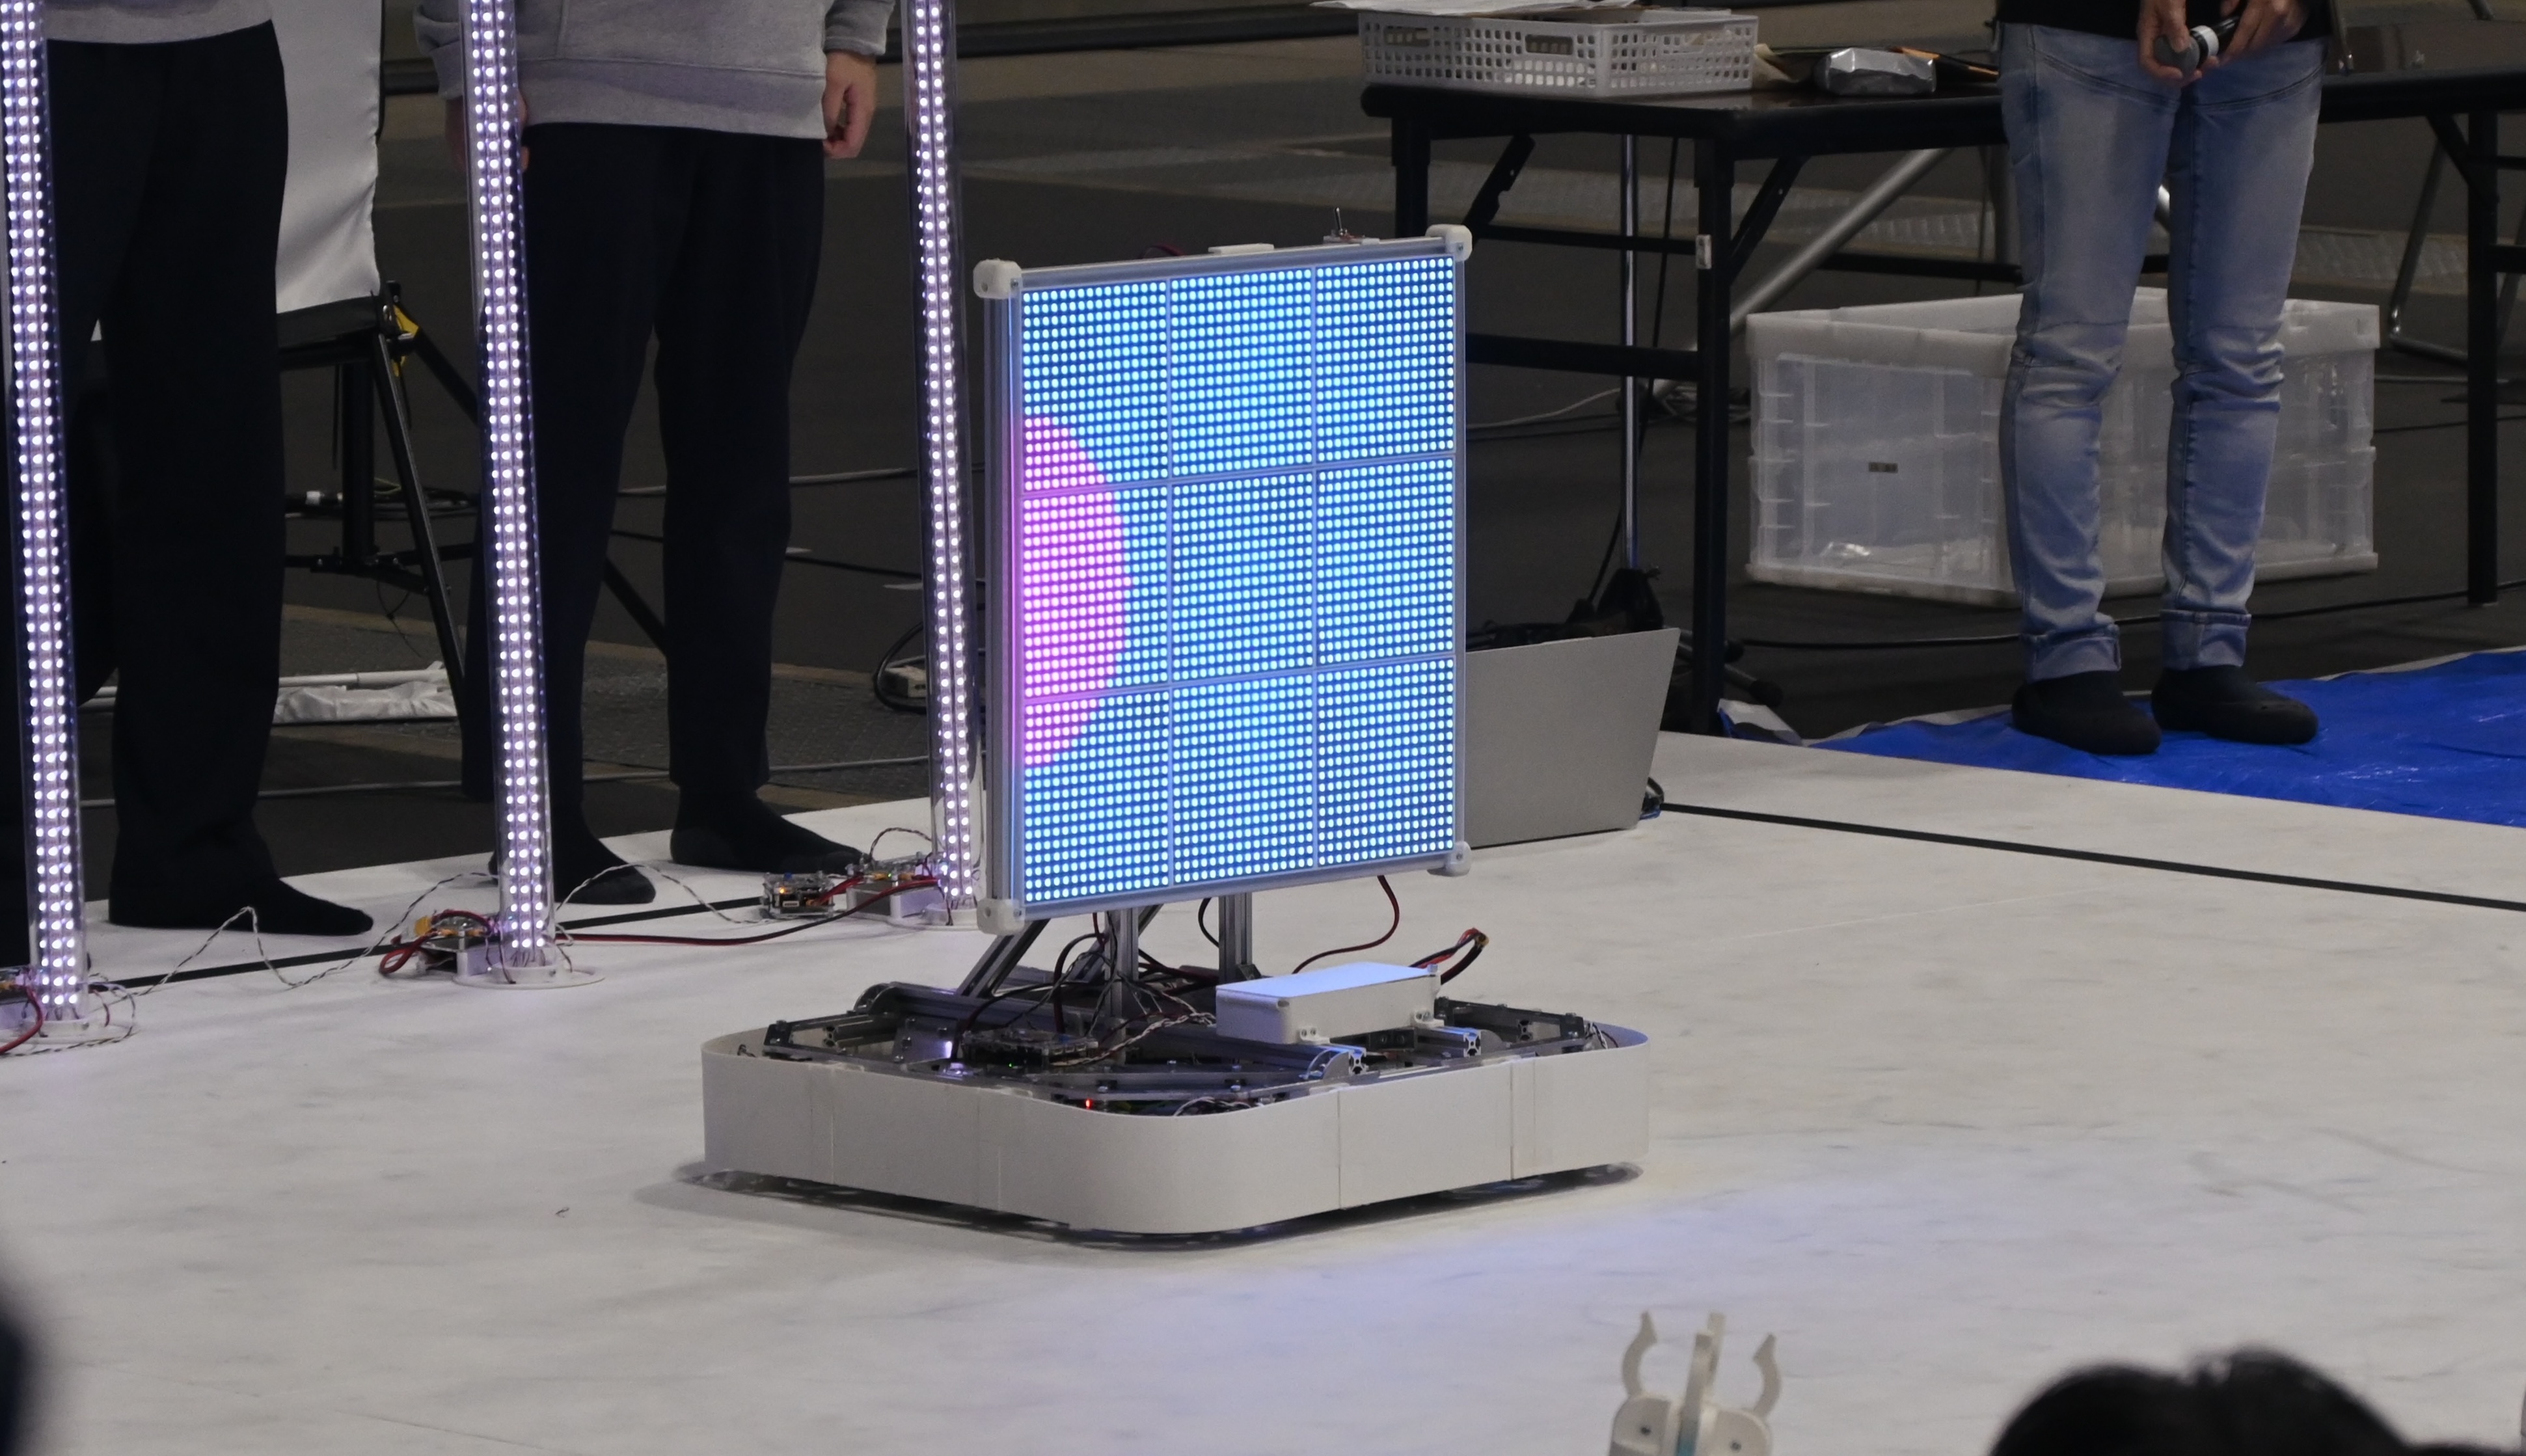
\includegraphics[width=0.8\columnwidth]{display.jpg}
\caption{過去に開発した自走式ディスプレイ}
\label{fig:display}
\end{figure}

\section{問題}
過去に開発した自走式ディスプレイでは、計算能力の低いマイクロコントローラーでレンダリングとLEDの駆動処理を行っていた(図\ref{fig:syuhou})ためディスプレイの表示内容に多くの制約があった。

マイクロコントローラーによるレンダリング処理では、複雑な画像処理が難しく、リアルタイムでインタラクションを行うためには、円の描画や、画像の拡大・縮小などの基本的な処理しか行えなかった。

使用しているマイコン内臓フルカラーLED(NeoPixel)は、数珠繋ぎに接続する必要があり、LEDの数が増えると、1フレームの描画にかかる時間が長くなり、フレームレートが低下してしまう問題もあった。しかし、マイコンによるLED制御では、特殊なプロトコル\cite{WS2812C2020V1}のため、チャンネルを増やすことは難しく、LEDの数を増やすこともできなかった。

\begin{figure}
\centering

\includegraphics[width=0.95\columnwidth]{syuhou.png}
\caption{手法の概要}
\label{fig:syuhou}
\end{figure}

\section{提案手法}
本稿では、図\ref{fig:syuhou}のようにレンダリング処理をSBC(Single Board Computer)に任せ、LEDの駆動処理をFPGAで行うことで、ディスプレイの表示内容の制約を解消する。LED駆動にFPGAを使用することで、LED制御モジュールの並列化により複数チャンネルを同時に制御することが可能になり、フレームレートを向上させることができる。

SBCは、レンダリング処理を行い、フレームバッファに書き込み、LinuxのSPIドライバを使用して、FPGAにフレームバッファの内容を送信する。

FPGAは、SPIクライアンモジュールを使用して、SBCからフレームバッファの内容を受信し、ダブルバッファに書き込む。そして、LED駆動モジュールがダブルバッファから読み出し、LEDを駆動する。ダブルバッファ使用することで、LED駆動中に表示内容が書き換わり、表示のティアリングを防ぐ。

\begin{figure}
\centering
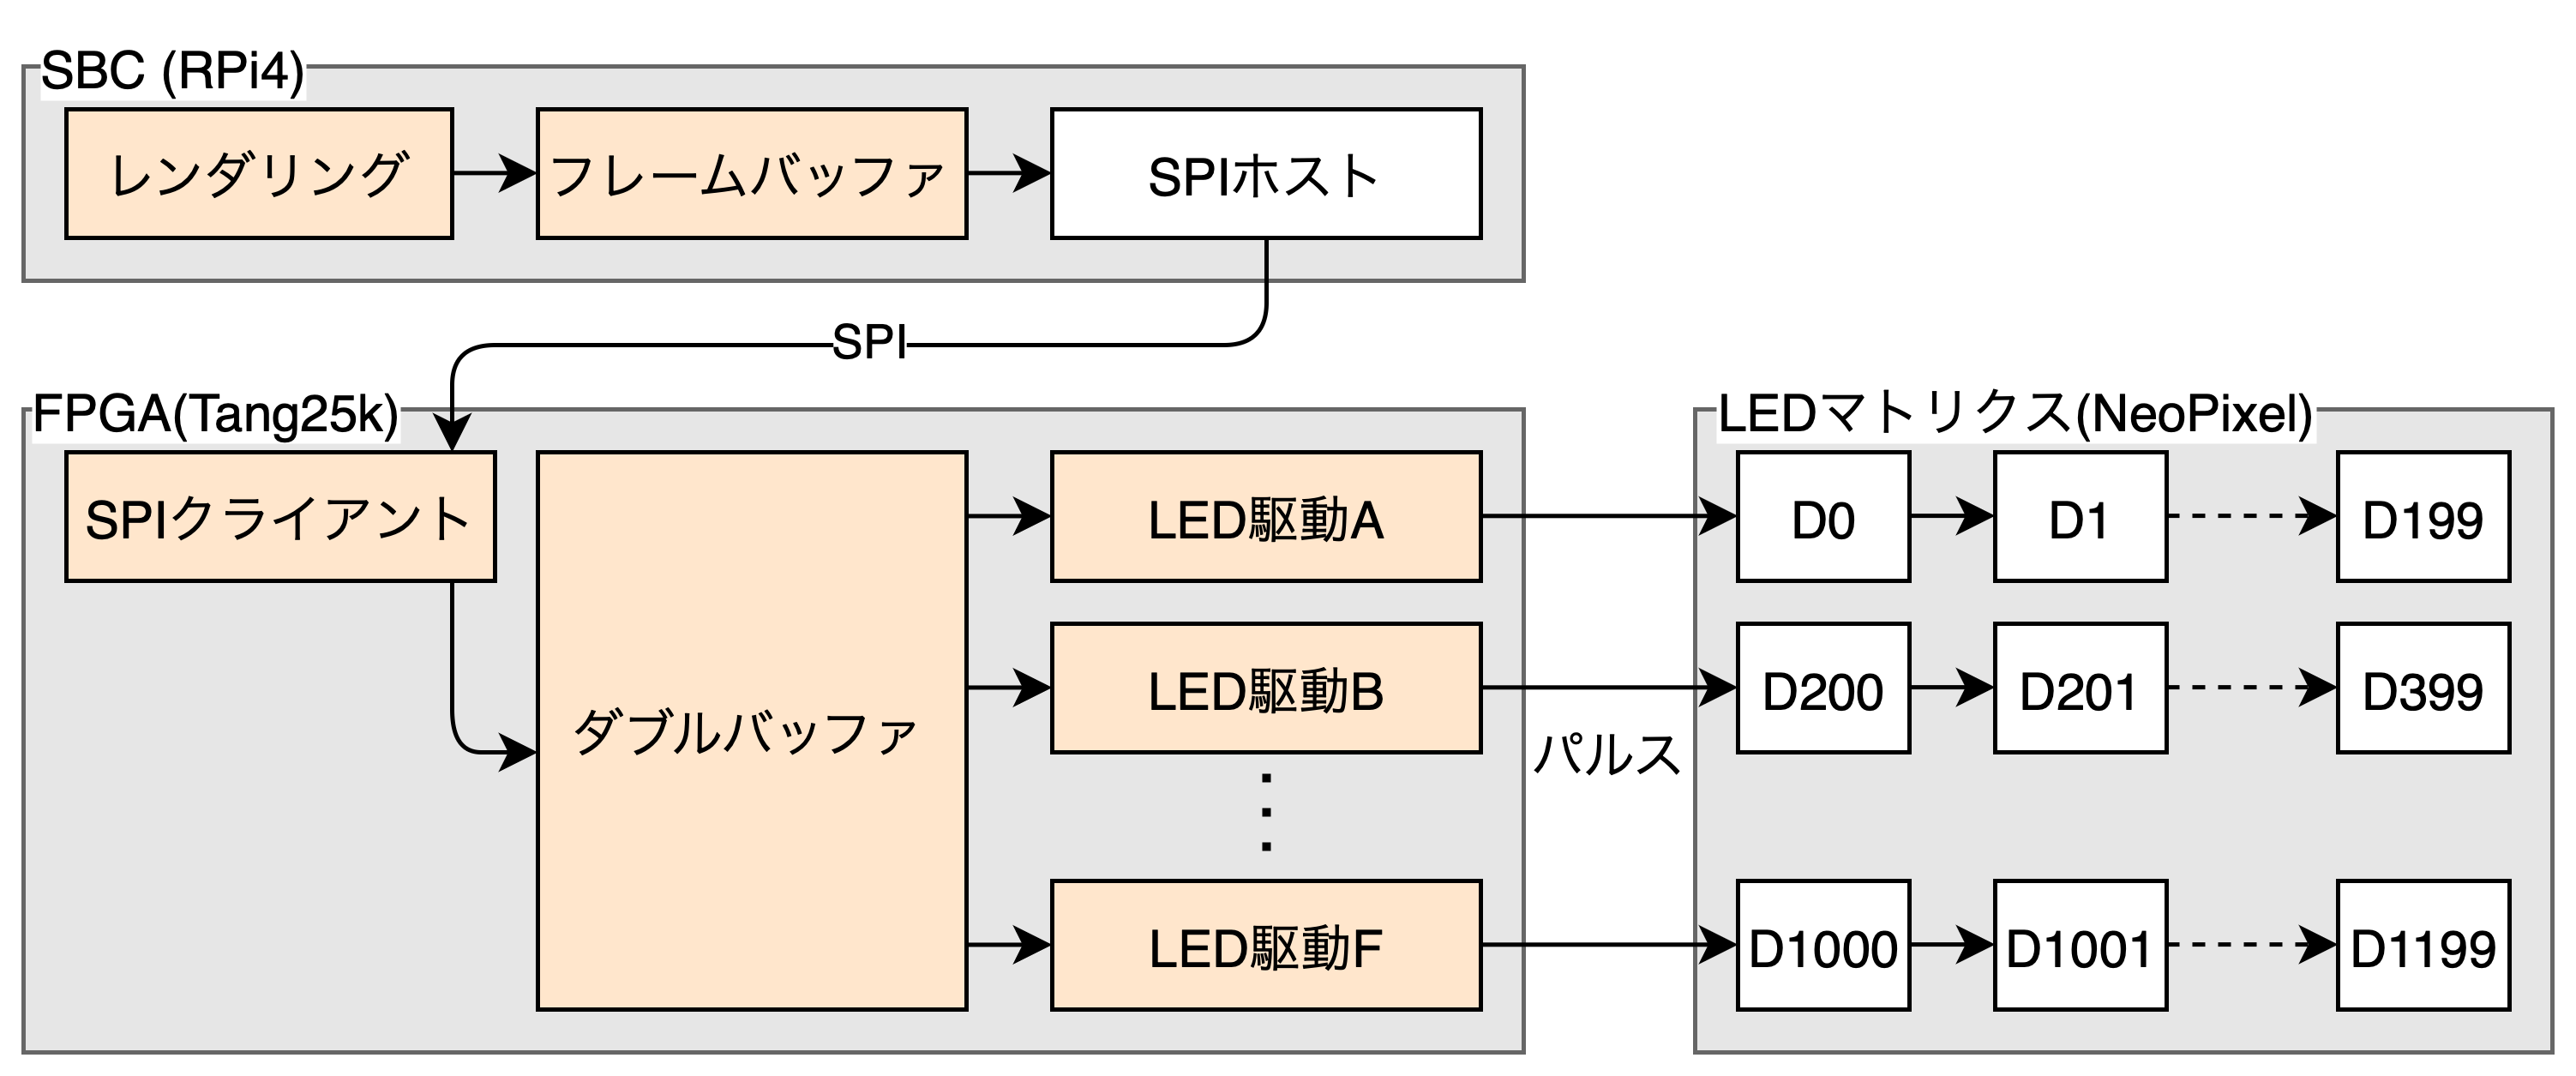
\includegraphics[width=0.95\columnwidth]{syuhou2.png}
\caption{提案手法(色付き部が筆者が実装した部分)}
\label{fig:syuhou2}
\end{figure}


\section{検証環境}
検証には、図\ref{fig:kensyo}に示すような環境を用意した。SBCには、Raspberry Pi 4 Model Bを使用し、FPGAには、TangPrimer25Kを使用した。また電源装置やロジックアナライザを接続し、SPI通信の動作を確認した。

実装には、FPGAのシミュレーション環境として、iVerilog、GTKWaveを使用した。合成には、GowinEDAを使用した。SBCには、C言語を使用して、SPI通信のテストプログラムを実装した。

\begin{figure}
\centering
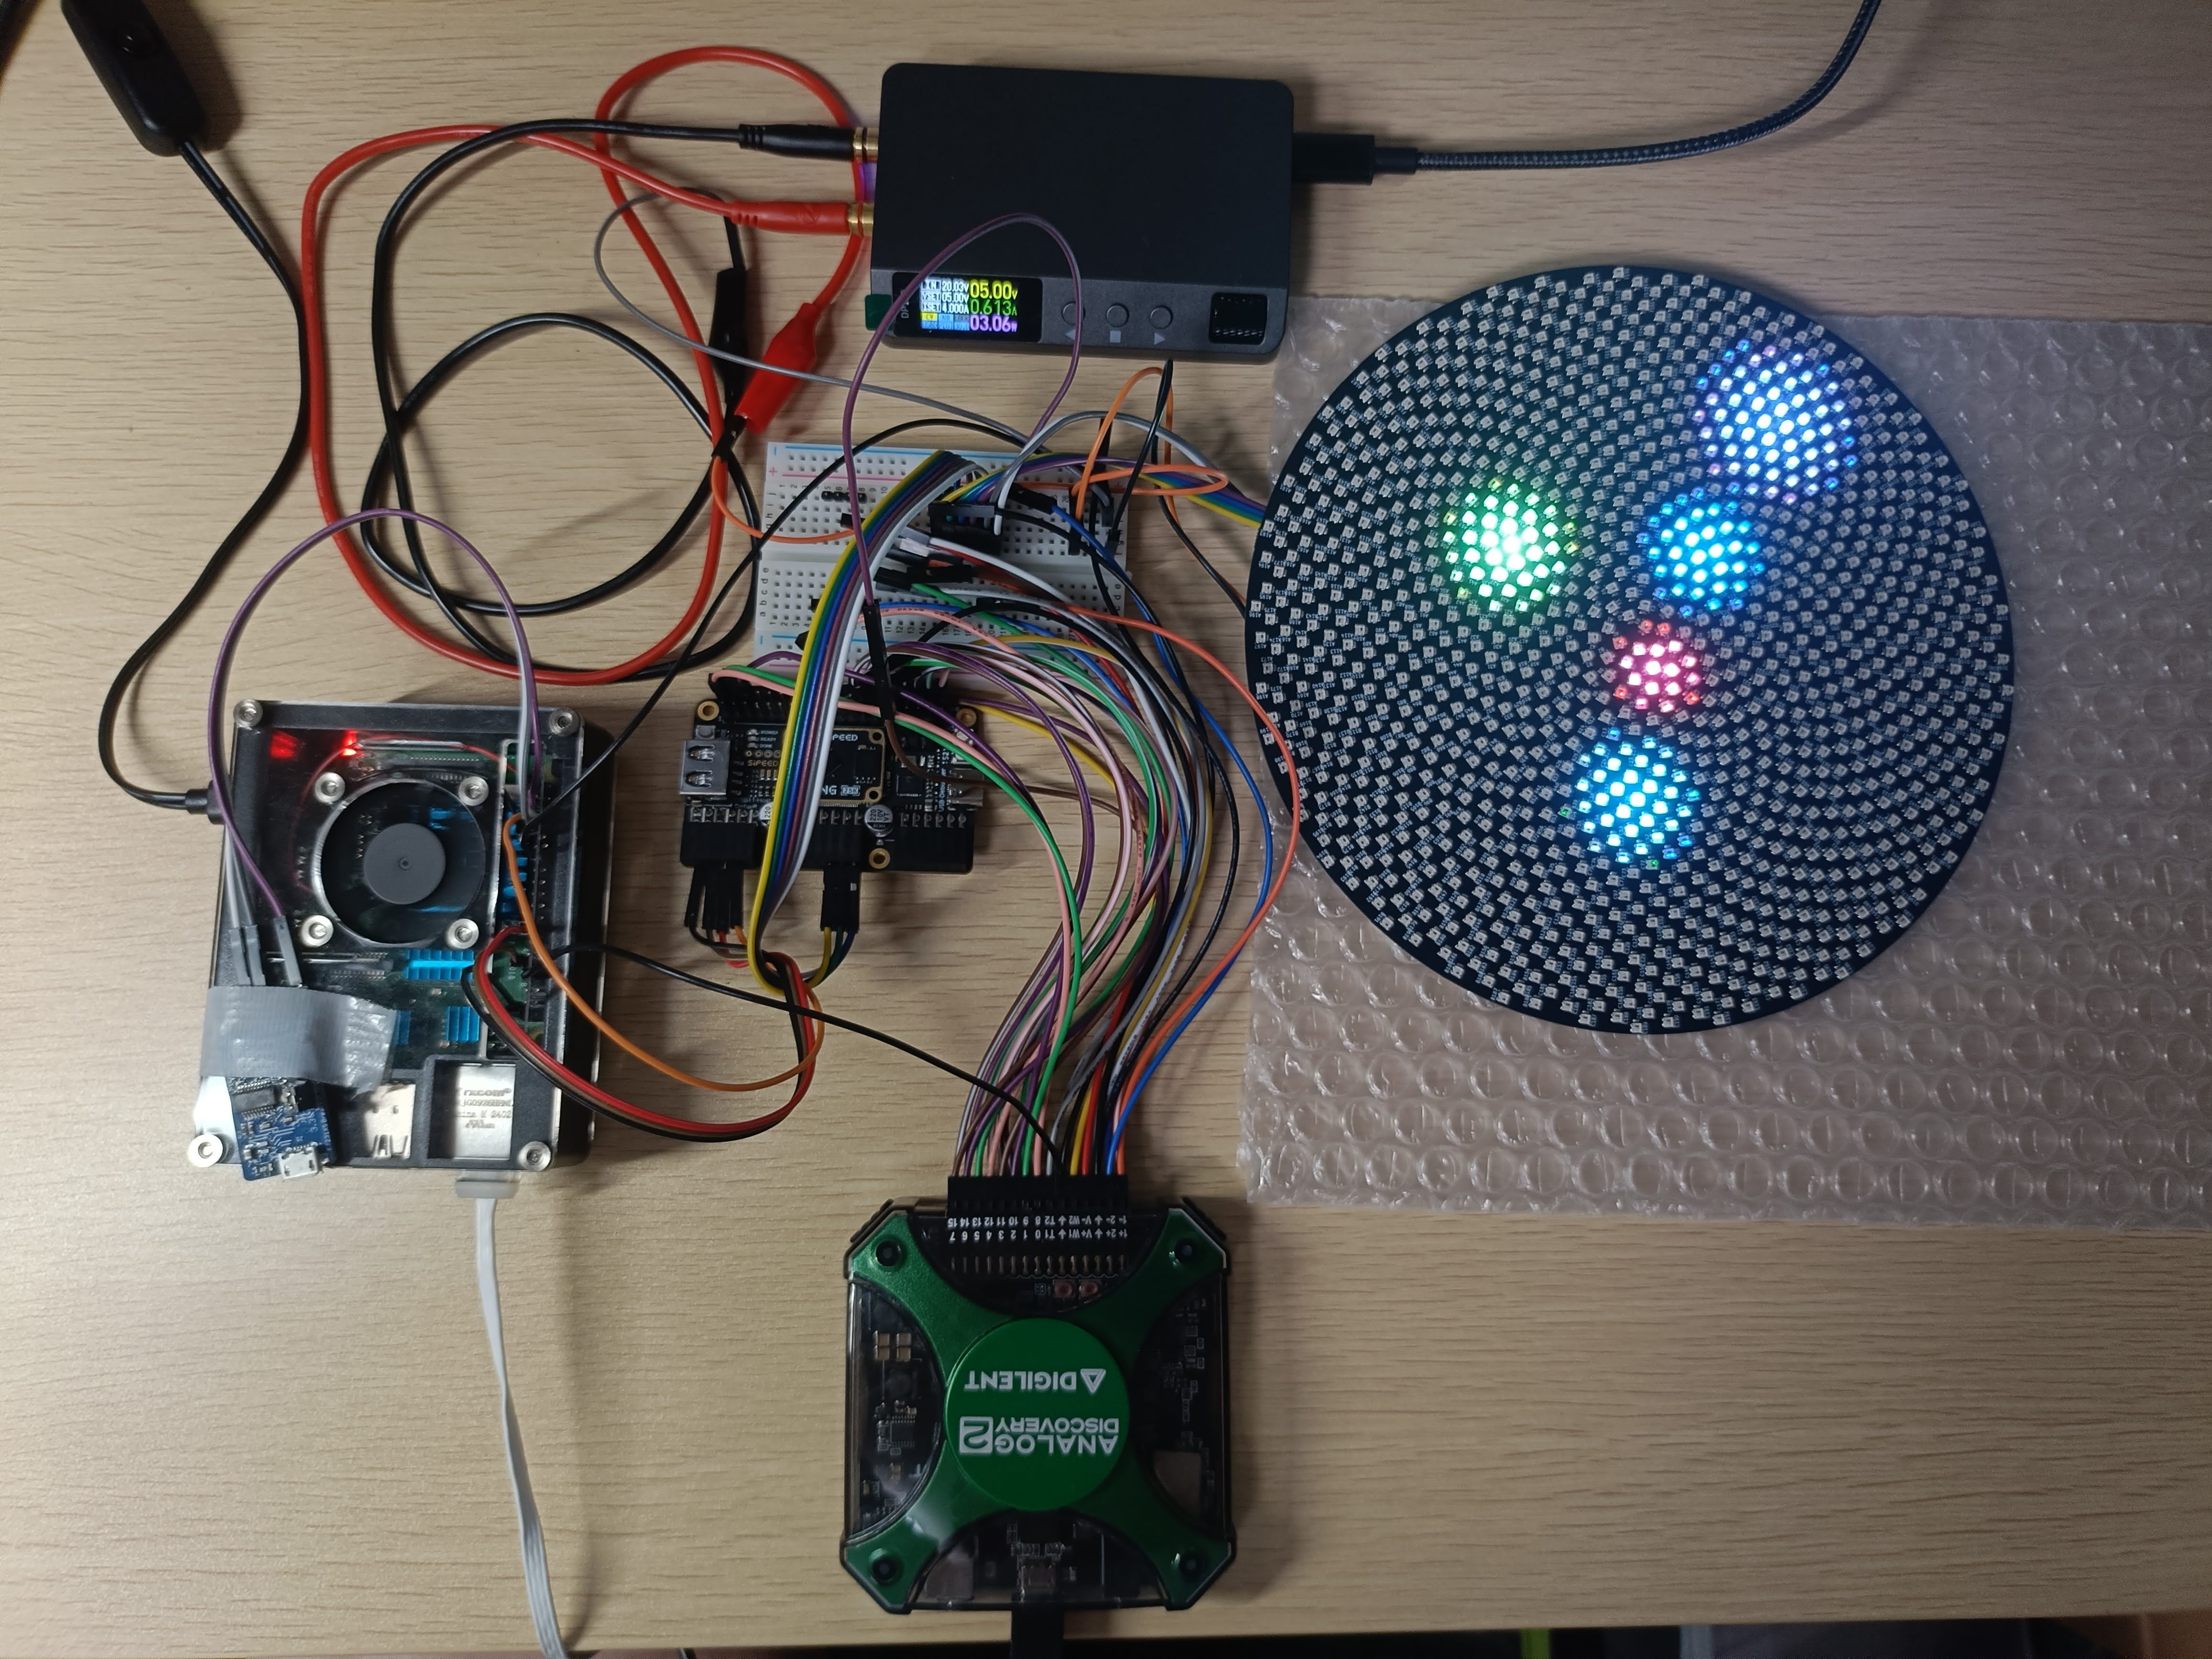
\includegraphics[width=0.8\columnwidth]{test.jpg}
\caption{検証環境}
\label{fig:kensyo}
\end{figure}

\section{動作検証}
図\ref{fig:dousa}に示すように、SBCとFPGAを組み合わせたシステムで、複数の円を同時に描画することができた。FPGAによるLED駆動処理により、フレームレートは約200fpsを達成し、リアルタイムでのインタラクションが可能になった。

\begin{figure}
\centering
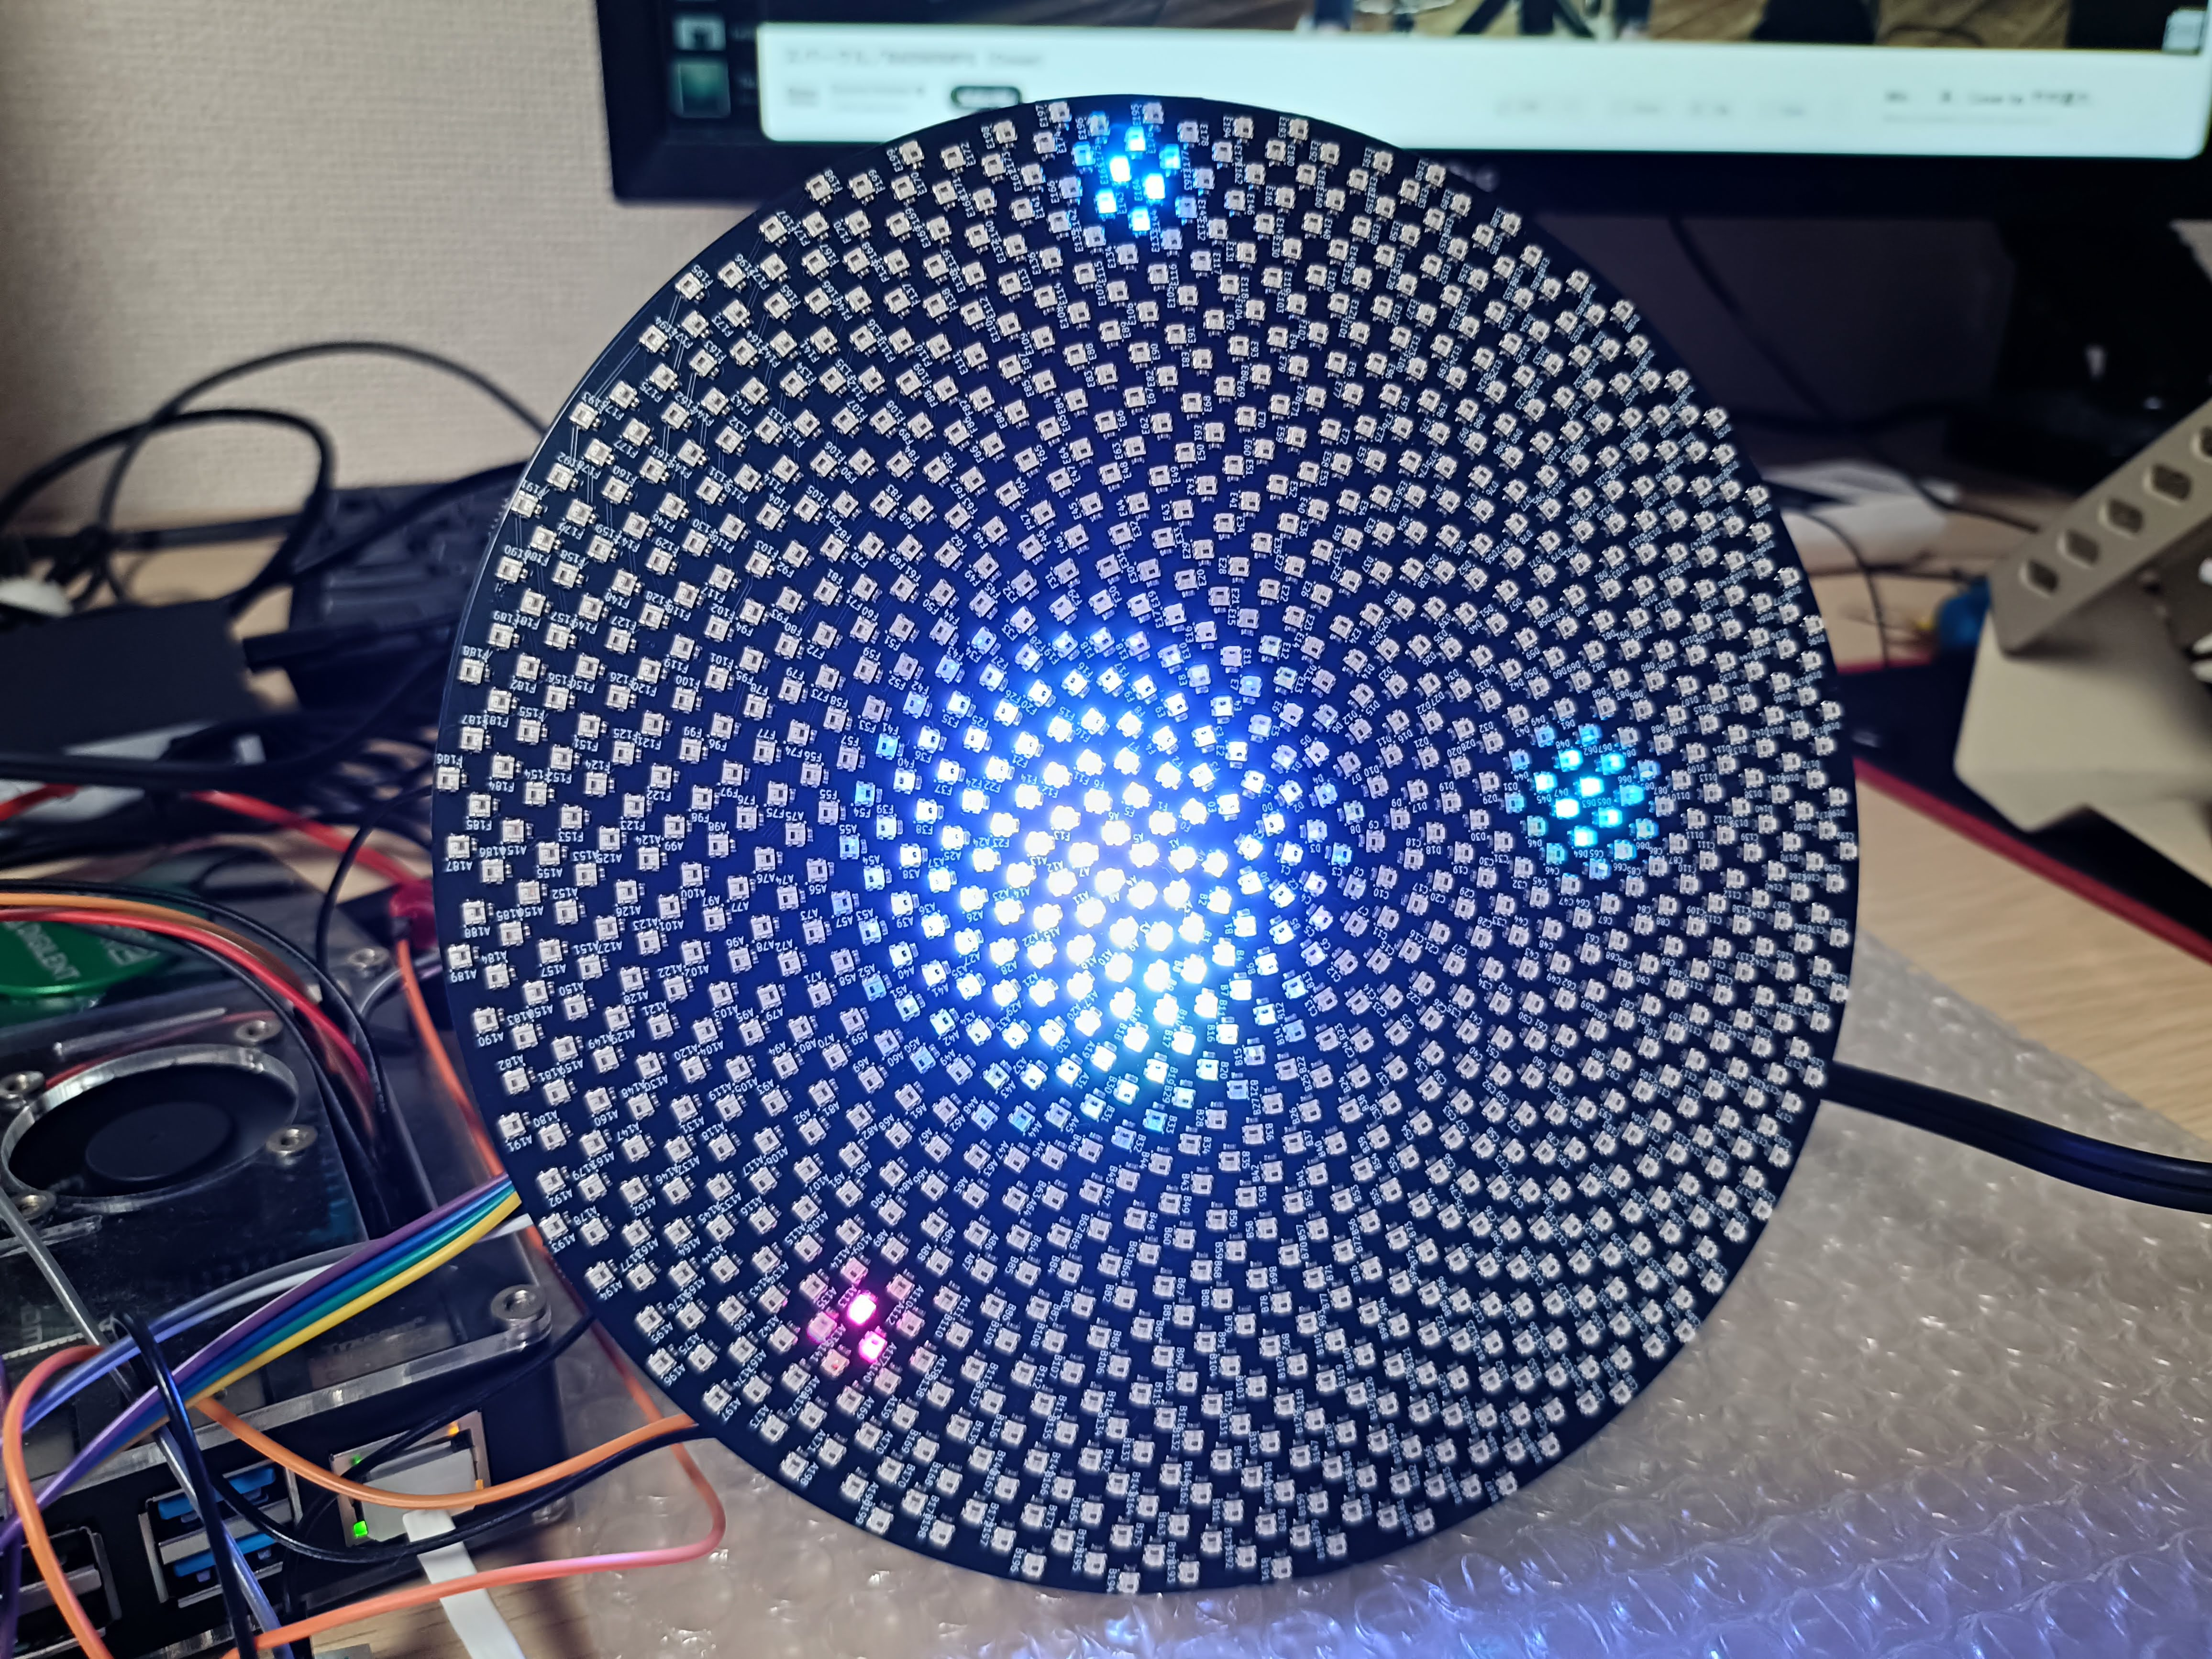
\includegraphics[width=0.8\columnwidth]{dousa.jpg}
\caption{動作している様子}
\label{fig:dousa}
\end{figure}

\section{まとめ}
本稿では、FPGAを使用した自走式ディスプレイのLEDマトリクスコントローラーの実装について述べた。FPGAを使用することで、LEDの駆動処理を高速化し、フレームレートを向上させることができた。これにより、ディスプレイの表示内容の制約を解消し、リアルタイムでのインタラクションが可能になった。

今後は、SBC側に複雑な画像処理や、3D表示などの機能を追加し、ディスプレイの表現力を向上させることを目指す。また、今回のシステムをPCB基板に実装し、小型化することで、開発している自走式ディスプレイに搭載することを目指す。

\printbibliography[title=参考文献]

\end{document}